\newpage
\section{Νευρωνικά Δίκτυα}
Τα νευρωνικά δίκτυα είναι στις μέρες μας το κυρίαρχο μοντέλο στη μηχανική μάθηση και μπορεί να λύσει και τους τρεις τύπους προβλημάτων που έχουμε δει (ταξινόμηση, παλινδρόμηση και ομαδοποίηση). Τα τεχνητά νευρωνικά δίκτυα δημιουργήθηκαν με
σκοπό να μιμηθούν τον τρόπο που λειτουργεί ο εγκέφαλος του ανθρώπου. Οι νευρώνες του εγκεφάλου μας λειτουργούν δημιουργώντας συνδέσεις με άλλους νευρώνες και όλοι μαζί συμβάλουν στην επεξεργασία ενός ηλεκτρικού σήματος που έρχεται από τον
εγκέφαλο το οποίο τελικά καταλήγει να είναι απλή καθημερινή πράξη για τον άνθρωπο (όπως για παράδειγμα να κουνήσει το χέρι του)\cite{nnip}.

Τα τεχνητά νευρωνικά δίκτυα προσπαθούν λοιπόν να αντιγράψουν αυτη ακριβώς την ιδιότητα. Ο σκοπός τους είναι να παίρνουν μια είσοδο και να παράγουν μία απάντηση. Για παράδειγμα θα μπορούσαμε σαν είσοδο να δώσουμε τις αιματολογικές εξετάσεις
ενός ανθρώπου και η έξοδος να είναι 0 ή 1 ανάλογα αν έχει μια ασθένεια ή όχι. Αυτό είναι ένα πρόβλημα δυαδικής ταξινόμησης αλλά θα μπορούσαμε να λύσουμε και πολλά άλλα προβλήματα και θα αναλύσουμε στην συνέχεια τις αλλαγές που πρέπει να
κάνουμε σε ένα νευρωνικό δίκτυο ανάλογα το πρόβλημα. Σε αυτή την ενότητα θα αναλύσουμε διάφορες έννοιες τις οποίες πρέπει να γνωρίζει κανείς αν θέλει να κατανοήσει τα νευρωνικά δίκτυα. Αυτές είναι\cite{nnav}:
\begin{itemize}
    \item Νευρώνας
    \item Επίπεδο
    \item Οπισθοδρόμηση (\en{back propagation})
    \item Συναρτήσεις ενεργοποίησης
    \item Συναρτήσεις σφάλματος
\end{itemize}

\subsection{Νευρώνας}
\subsection{Επίπεδο}
\subsection{Οπισθοδρόμηση}
\subsection{Συναρτήσεις ενεργοποίησης}
Οι συναρτήσεις ενεργοποίησης είναι ένα πολύ σημαντικό κομμάτι των νευρωνικών δικτύων διότι προσφέρουν μη γραμμικότητα (επιθυμητή) στο σύστημά μας. Για να καταλάβουμε καλύτερα τι σημαίνει αυτό θα δούμε ένα παράδειγμα\cite{nnactmlm}:

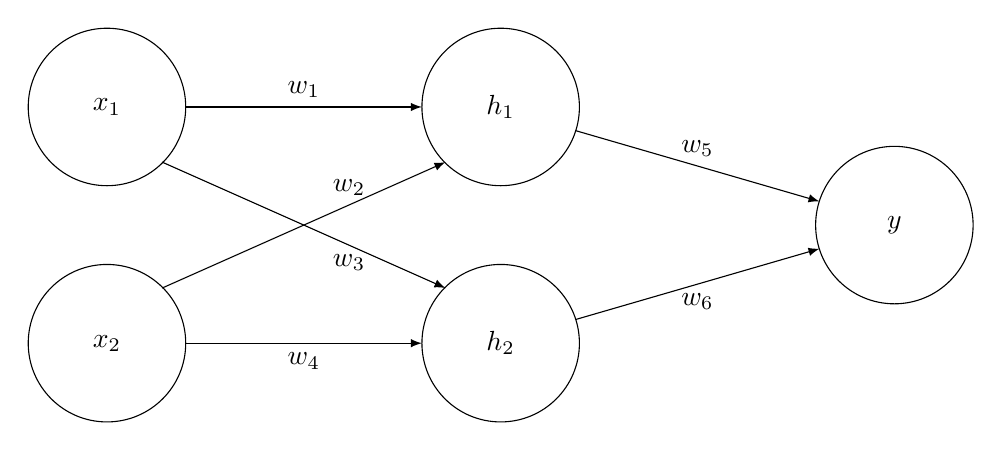
\begin{tikzpicture}
    \draw (0,0) circle (1) node{$x_2$};
    \draw (0,3) circle (1) node{$x_1$};
    \draw (5,0) circle (1) node{$h_2$};
    \draw (5,3) circle (1) node{$h_1$};
    \draw (10,1.5) circle (1) node{$y$};

    \draw[-latex] (1,0) -- (4,0) node[midway, below]{$w_4$};
    \draw[-latex] (1,3) -- (4,3) node[midway, above]{$w_1$};

    \draw[-latex] (0.7,0.7) -- (4.3,2.3) node[midway, above right=7]{$w_2$};
    \draw[-latex] (0.7,2.3) -- (4.3,0.7) node[midway, below right=7]{$w_3$};

    \draw[-latex] (5.95,2.7) -- (9.05,1.8) node[midway, above]{$w_5$};
    \draw[-latex] (5.95,0.3) -- (9.05,1.2) node[midway, below]{$w_6$};
\end{tikzpicture}

Βλεπουμε ότι η είσοδος με την έξοδο συνδέονται μέσω ενός κρυφού επιπέδου (\en{dense}) όπου:
\begin{gather*}
    h_1=w_1\times x_1+w_2\times x_2 \\
    h_2=w_3\times x_1+w_4\times x_2 \\
    y=w_5\times h_1+w_6\times h_2 \\
\end{gather*}
Αν αναλύσουμε λοιπόν τον τύπο του $y$ θα πάρουμε:
$$y=w_1(w_5\times x_1+w_2\times x_2) + w_6(w_3\times x_1+w_4\times x_2)$$
Που τελικά γίνεται:
$$y=(w_1w_5+w_3w_6)\times x_1+(w_2w_5+w_4w_6)\times x_2$$
Τα $w$ είναι σταθεροί αριθμοί οπότε τελικά ενώ έχουμε ένα κρυφό επίπεδο ανάμεσα στην είσοδο και στην έξοδο αυτές συνδέονται και πάλι με γραμμική σχέση. Το ίδιο θα συνέβαινε και για πολλαπλά κρυφά επίπεδα με πολλούς νευρώνες. Αυτό για το
δίκτυο μας σημαίνει ότι μπορεί να προσεγγίσει δεδομένα που ακολουθούν επίσης μια γραμμική σχέση. Τα δεδομένα όμως συνήθως δεν έχουν τέτοια συμπεριφορά. Για να λύσουμε αυτό το πρόβλημα δημιουργήθηκαν οι συναρτήσεις ενεργοποίησης. Στο
παράδειγμά μας μπορούμε να προσθέσουμε μις συνάρτηση ενεργοποίησης αμέσως μετά το κρυφό επίπεδο. Έτσι τελικά η έξοδος θα είναι:
$$y=w_5\times f_A(h_1)+w_6\times f_A(h_2)$$
Όπου $f_A$ η συνάρτηση ενεργοποίησης. Παρατηρούμε ότι η είσοδος δεν μπορεί πλέον να συνδεθεί γραμμικά με την έξοδο και άρα έχουμε πετύχει τον στόχο μας.

Υπάρχουν πολλές συναρτήσεις ενεργοποίησης και όλες έχουν τα πλεονεκτήματα και τα μειονεκτήματα τους. Εμεις θα αναλύσουμε κάποιες από τις πιο γνωστές οι οποίες χρησιμοποιούνται σχεδόν πάντα στα νευρωνικά δίκτυα.

\begin{tikzpicture}
\begin{axis}[axis lines=middle, xlabel=$x$, ylabel=$y$, title=\en{step function}, xmin = -5, xmax=5, ymin=0, ymax=2, xtick={-5,-4,...,5}, ytick={0,1,2}]
    \addplot[color=red, domain=0:10]{1};
    \addplot[color=red, domain=-10:0]{0};
\end{axis}
\end{tikzpicture}

\begin{tikzpicture}
\begin{axis}[axis lines=middle, xlabel=$x$, ylabel=$y$, title=\en{ReLU function}, xmin = -5, xmax=5, ymin=0, ymax=5, xtick={-5,-4,...,5}, ytick={0,1,...,5}, axis equal]
    \addplot[color=red, domain=0:10]{x};
    \addplot[color=red, domain=-10:0]{0};
\end{axis}
\end{tikzpicture}

\begin{tikzpicture}
    \begin{axis}[axis lines=middle, xlabel=$x$, ylabel=$y$, title=\en{leaky ReLU function}, xmin = -5, xmax=5, ymin=0, ymax=5, xtick={-5,-4,...,5}, ytick={0,1,...,5}, axis equal]
        \addplot[color=red, domain=0:10]{x};
        \addplot[color=red, domain=-10:0]{0.1*x};
\end{axis}
\end{tikzpicture}

\begin{tikzpicture}
    \begin{axis}[axis lines=middle, xlabel=$x$, ylabel=$y$, title=\en{ELU function}, xmin = -5, xmax=5, ymin=0, ymax=5, xtick={-5,-4,...,5}, ytick={0,1,...,5}, axis equal]
        \addplot[color=red, domain=0:10]{x};
        \addplot[color=red, domain=-10:0]{(exp(x)-1)};
\end{axis}
\end{tikzpicture}

\begin{tikzpicture}
    \begin{axis}[axis lines=middle, xlabel=$x$, ylabel=$y$, title=\en{SELU function}, xmin = -5, xmax=5, ymin=-5, ymax=5, xtick={-5,-4,...,5}, ytick={0,1,...,5}, axis equal]
        \addplot[color=red, domain=0:10]{x};
        \addplot[color=red, domain=-10:0]{2*(exp(x)-1)};
\end{axis}
\end{tikzpicture}

\begin{tikzpicture}
    \begin{axis}[axis lines=middle, xlabel=$x$, ylabel=$y$, title=\en{GELU function}, xmin = -5, xmax=5, ymin=0, ymax=5, xtick={-5,-4,...,5}, ytick={0,1,...,5}, axis equal]
        \addplot[color=red]{0.5*x*(1+tanh(sqrt(2)/pi*(x+0.044715*x^3)))};
\end{axis}
\end{tikzpicture}

\begin{tikzpicture}
\begin{axis}[axis lines=middle, xlabel=$x$, ylabel=$y$, title=\en{sigmoid function}, xmin = -5, xmax=5, ymin=0, ymax=2, xtick={-5,-4,...,5}, ytick={0,1,2}]
    \addplot[color=red]{exp(x)/(exp(x)+1)};
\end{axis}
\end{tikzpicture}

\begin{tikzpicture}
\begin{axis}[axis lines=middle, xlabel=$x$, ylabel=$y$, title=\en{swish function}, xmin = -5, xmax=5, ymin=-2, ymax=2, xtick={-5,-4,...,5}, ytick={0,1,2}]
    \addplot[color=red]{x/(exp(-x)+1)};
\end{axis}
\end{tikzpicture}

\begin{tikzpicture}
    \begin{axis}[axis lines=middle, xlabel=$x$, ylabel=$y$, title=\en{tanh function}, xmin = -5, xmax=5, ymin=-2, ymax=2, xtick={-5,-4,...,5}, ytick={-2,-1,...,2}]
        \addplot[color=red]{tanh(x)};
    \end{axis}
    \end{tikzpicture}
\subsection{Συναρτήσεις σφάλματος}